% 独自のコマンド

% ■ 謝辞
%  \begin{acknowledgment} 〜 \end{acknowledgment}

% ■ 文献リスト
%  \begin{bib}[100] 〜 \end{bib}


\newif\ifjapanese

\japanesetrue  % 論文全体を日本語で書く(英語で書くならコメントアウト)

\ifjapanese
  \documentclass[a4j,twoside,openright,11pt,dvipdfmx]{ujreport} % 両面印刷の場合。余白を綴じ側に作って右起こし。
  %\documentclass[a4j,11pt,dvipdfmx]{ujreport}                  % 片面印刷の場合。
  \renewcommand{\bibname}{参考文献}
  \newcommand{\acknowledgmentname}{謝辞}
\else
  \documentclass[a4paper,11pt]{report}
  \newcommand{\acknowledgmentname}{Acknowledgment}
\fi

% packages
\usepackage{thesis}
\usepackage{ascmac}
\usepackage{graphicx}
\usepackage{multirow}
\usepackage{url}
\usepackage{booktabs}

\bibliographystyle{jplain}

\bindermode  % バインダー用余白設定

% 日本語情報(必要なら)
\jprogram    {筑波大学大学院博士前期課程}
\jcourse     {数理物質科学研究科修士論文}
\jtitle      {修士論文題目}    % 改行する場合は\\を入れる
\jauthor     {著者氏名}
\jmajor      {○○○専攻}
\jdate       {2021年2月}
\jsupervisor {○○○○○○}

% 英語情報(必要なら)
\eprogram    {Master's Program in Name of Major Field}
\ecourse     {Submitted to the Graduate School of\\Pure and Applied Sciences\\in Partial Fulfillment of the Requirements\\for the Degree of Master of Name of Degree\\ \\at the\\University of Tsukuba}
\etitle      {Title of Master Thesis}    % 改行する場合は\\を入れる
\eauthor     {Name of Author}
\emajor      {Name of Major Field}
\edate       {Feburuary 2021}
\esupervisor {○○○○○○}

% 画像のpath
\graphicspath{{../graphics/}}


\begin{document}

\ifjapanese
  \jmaketitle    % 表紙(日本語)
\else
  \emaketitle    % 表紙(英語)
\fi

\begin{abstract} \baselineskip = 1cm
    いい感じの概要.いい感じの概要.いい感じの概要.いい感じの概要.いい感じの概要.いい感じの概要.いい感じの概要.いい感じの概要.いい感じの概要.いい感じの概要.いい感じの概要.いい感じの概要.いい感じの概要.いい感じの概要.いい感じの概要.いい感じの概要.いい感じの概要.いい感じの概要.いい感じの概要.いい感じの概要.いい感じの概要.いい感じの概要.いい感じの概要.いい感じの概要.
\end{abstract}


\tableofcontents  % 目次
\listoffigures    % 表目次
\listoftables     % 図目次

\pagenumbering{arabic}

% 本文
\chapter{序論} \label{chap:introduction}

\begin{figure}[htbp]
  \begin{center}
    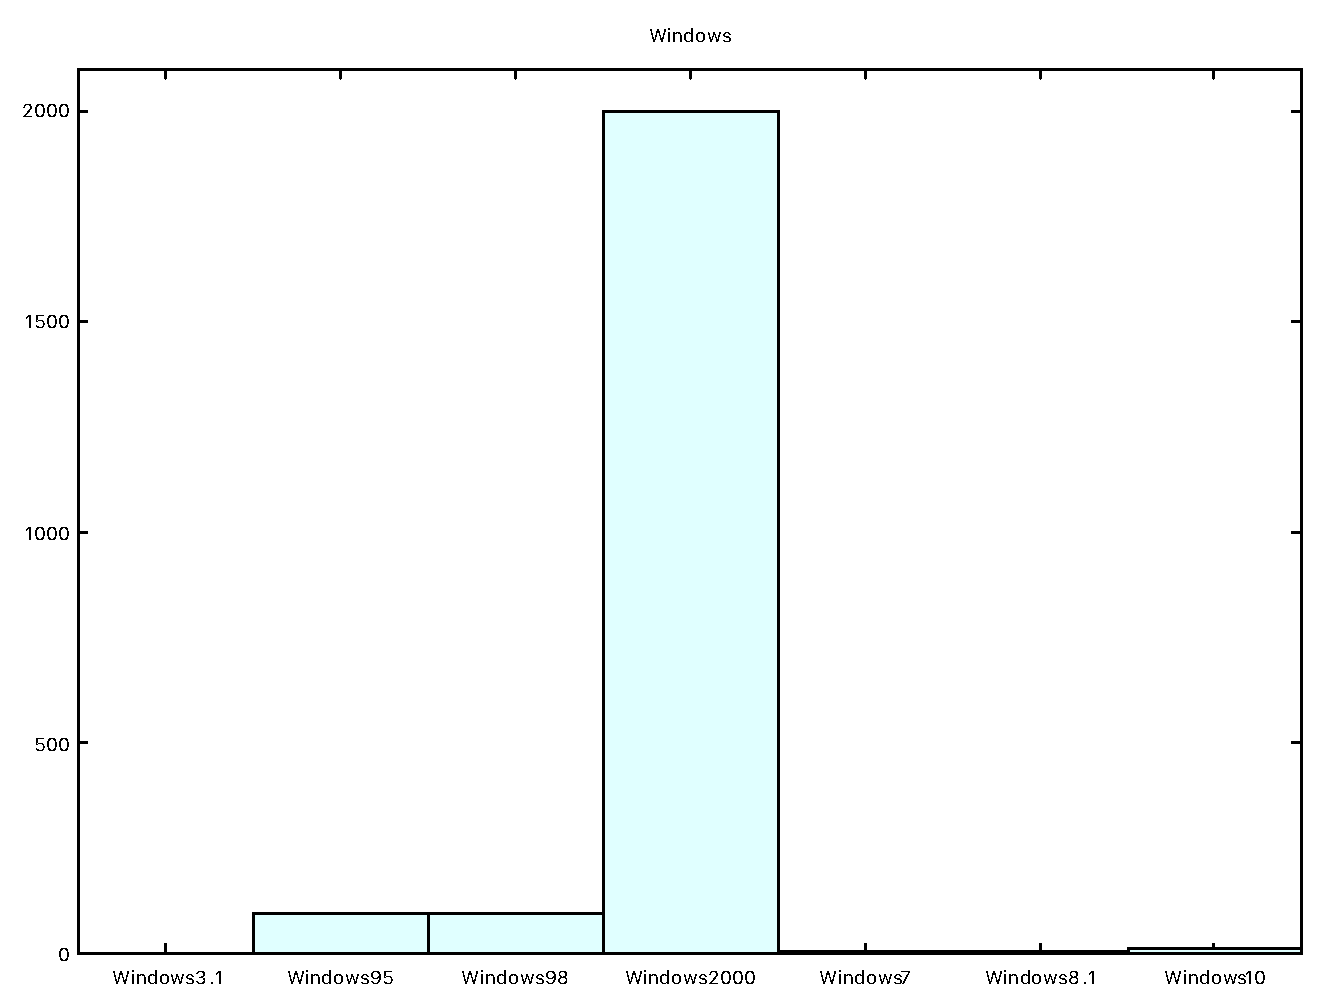
\includegraphics[width=\textwidth]{Windows.pdf}
  \end{center}
  \caption{Windows OS}
  \label{fig:Windows}
\end{figure}

\begin{table}[htbp]
  \begin{center}
    \begin{tabular}{cccc}\toprule
      バージョン & コードネーム & 読み方 & リリース\\ \midrule
      Mac OS X 10.0 & Cheetah & チーター & 2001年3月\\
      Mac OS X 10.1 & Puma & ピューマ & 2001年9月\\
      Mac OS X 10.2 & Jaguar & ジャガー & 2002年8月\\
      Mac OS X 10.3 & Panther & パンサー & 2003年10月\\
      Mac OS X 10.4 & Tiger & タイガー & 2005年4月\\
      Mac OS X 10.5 & Leopard & レパード & 2007年10月\\
      Mac OS X 10.6 & Snow Leopard & スノー レパード & 2009年8月\\
      Mac OS X 10.7 & Lion & ライオン & 2011年7月\\
      OS X 10.8 & Mountain Lion & マウンテン ライオン & 2012年7月\\
      OS X 10.9 & Mavericks & マーベリックス & 2013年10月\\
      OS X 10.10 & Yosemite & ヨセミテ & 2014年10月16日\\
      OS X 10.11 & El Capitan & エル キャピタン & 2015年10月1日\\
      macOS 10.12 & Sierra & シエラ & 2016年9月20日\\
      macOS 10.13 & High Sierra & ハイ シエラ & 2017年9月25日\\
      macOS 10.14 & Mojave & モハベ & 2018年9月25日\\
      macOS 10.15 & Catalina & キャタリナ & 2019年10月7日\\
      macOS 11.0 & Big Sur & ビッグサー & 2020年11月12日\\ \bottomrule
    \end{tabular}
  \end{center}
  \caption{Mac OS}
  \label{tb:Mac}
\end{table}

第\ref{chap:introduction}章しかないけど許して.図\ref{fig:Windows}.表\ref{tb:Mac}.\par
Tensor Renormalization Group\cite{PhysRevLett.99.120601}.
% \include{02}
% \include{03}
% ...


\begin{acknowledgment}

    お世話になった人には感謝しましょう.

\end{acknowledgment}
  % 謝辞。要独自コマンド、include先参照のこと

\begin{bib}[100]
% BibTeXを使う場合
\bibliography{main}

%\begin{thebibliography}{#1}
%
%  \bibitem{参照用名称}
%    著者名: 
%    \newblock 文献名,
%    \newblock 書誌情報,出版年.
%
% \bibitem{hoge09}
%   ほげ山太郎,ほげ山次郎:
%   \newblock ほげほげ理論のHCI分野への応用,
%   \newblock ほげほげ学会論文誌,Vol.31,No.3,pp.194-201,2009.
% 
% \bibitem{hoge08}
%   Taro Hogeyama, Jiro Hogeyama:
%   \newblock The Theory of Hoge,
%   \newblock {\it The Proceedings of The Hoge Society}, 2008.
%	
%\end{thebibliography}

\end{bib}
    % 参考文献。要独自コマンド、include先参照のこと
\appendix
\chapter{付録の例}

付録を無理矢理出力させるため、てきとうなことを書く。

\section{ほげ}

コマンドは本文と一緒。

\subsection{ふー}

本文と一緒。

\section{ほげほげ}

本文と一緒。

\subsection{ふーふー}

本文と一緒。
    % 付録

\end{document}
